% !TeX program = xelatex
\documentclass{beamer}
\usepackage{xeCJK}
\usepackage{bookmark}
% 图片路径
\graphicspath{{Figures/}}
% 设置主题
\usetheme{Berkeley}
\usecolortheme{beaver}
\setbeamercolor{title in sidebar}{fg=black}
\setbeamercolor{section in sidebar shaded}{fg=black}
\usefonttheme{serif}
% 报告基本信息
\logo{\includegraphics[height=0.09\textwidth]{whulogo.eps}}
\title[Graph Embedding]{图表示学习}
\author[S. Zhou]{Zhou Shen}
\institute{School of Computer Science, Wuhan University}
\date{\today}

\begin{document}
% -----------------------------------------首页-----------------------------------------
\begin{frame}
    \titlepage
\end{frame}
% ----------------------------------------目录页----------------------------------------
\begin{frame}{Outline}
    \tableofcontents
\end{frame}
% ---------------------------------------Word2Vec---------------------------------------
\section{Word2Vec}
% one-hot encoding
\begin{frame}{Word2Vec}
    \framesubtitle{One-Hot Encoding}
    \centering\includegraphics[height=5cm]{one_hot.png}
\end{frame}
% one-word context
\begin{frame}{Word2Vec}
    \framesubtitle{One-Word Context}
    \centering\includegraphics[height=4cm]{word2vec_1.pdf}
    \begin{equation}
        \mathbf{h}=\mathbf{W}^{T} \mathbf{x}=\mathbf{W}_{(k, \cdot)}^{T}:=\mathbf{v}_{w_{I}}^{T}, u_j=\mathbf{v}_{w_j}^{\prime}h
    \end{equation}
    \begin{equation}
        p\left(w_{j} \mid w_{I}\right)=y_{j}=\frac{\exp \left(u_{j}\right)}{\sum_{j^{\prime}=1}^{V} \exp \left(u_{j^{\prime}}\right)}
    \end{equation}
\end{frame}
% Objective Function
\begin{frame}{Word2Vec}
    \framesubtitle{Objective Function}
    \begin{equation}
        \begin{aligned}
        \max p\left(w_{O} \mid w_{I}\right) &=\max y_{j^{*}} \\
        &=\max \log y_{j^{*}} \\
        &=u_{j^{*}}-\log \sum_{j^{\prime}=1}^{V} \exp \left(u_{j^{\prime}}\right):=-E
        \end{aligned}
    \end{equation}
    \begin{alertblock}{常用变形}
        $\min E=-u_{j^{*}}+\log \sum_{j^{\prime}=1}^{V} \exp \left(u_{j^{\prime}}\right)$
    \end{alertblock}
\end{frame}
% CBOW
\begin{frame}{Word2Vec}
    \framesubtitle{CBOW}
    \begin{columns}
        % 第一列
        \begin{column}{0.4\textwidth}
            \centering\includegraphics[height=6cm]{word2vec_2.pdf}
        \end{column}
        % 第二列
        \begin{column}{0.6\textwidth}
            $$\mathbf{h} = \frac{1}{C}(\mathbf{v}_{w_1} + \mathbf{v}_{w_2} + \cdots + \mathbf{v}_{w_C})^T$$
            $$
            \begin{aligned}
                E &=-\log p\left(w_{O} \mid w_{I, 1}, \cdots, w_{I, C}\right) \\
                &=-u_{j^{*}}+\log \sum_{j^{\prime}=1}^{V} \exp \left(u_{j^{\prime}}\right) \\
            \end{aligned}
            $$
        \end{column}
    \end{columns}
\end{frame}
% Skip-Gram
\begin{frame}{Word2Vec}
    \framesubtitle{Skip-Gram}
    \begin{columns}
        % 第一列
        \begin{column}{0.4\textwidth}
            \centering\includegraphics[height=6cm]{word2vec_3.pdf}
        \end{column}
        % 第二列
        \begin{column}{0.6\textwidth}
            $$
            \begin{aligned}
            E &=-\log p\left(w_{O, 1}, w_{O, 2}, \cdots, w_{O, C} \mid w_{I}\right) \\
            &=-\log \prod_{c=1}^{C} \frac{\exp \left(u_{c, j_{c}^{*}}\right)}{\sum_{j^{\prime}=1}^{V} \exp \left(u_{j^{\prime}}\right)} \\
            &=-\sum_{c=1}^{C} u_{j_{c}^{*}}+C \cdot \log \sum_{j^{\prime}=1}^{V} \exp \left(u_{j^{\prime}}\right)
            \end{aligned}
            $$
        \end{column}
    \end{columns}
\end{frame}
% Hierarchical Softmax
\begin{frame}{Word2Vec}
    \framesubtitle{Hierarchical Softmax}
    \centering\includegraphics[height=4cm]{word2vec_4.pdf}
    $$
        p\left(w=w_{O}\right)=\prod_{j=1}^{L(w)-1} \sigma\left([ n(w, j+1)=\operatorname{ch}(n(w, j)) ] \cdot \mathbf{v}_{n(w, j)}^{\prime}{ }^{T} \mathbf{h}\right)
    $$
\end{frame}
% Negative Sample
\begin{frame}{Word2Vec}
    \framesubtitle{Negative Sample}
    1. 词频计算
    $$
        weight(w_i) = \frac{count(w_i)^{0.75}}{\sum_{j}^{V} count(w_j)^{0.75}}
    $$
    2. 目标函数
    $$
        E=-\log \sigma\left(\mathbf{v}_{w_{O}}^{\prime}{ }^{T} \mathbf{h}\right)-\sum_{w_{j} \in \mathcal{W}_{\mathrm{neg}}} \log \sigma\left(-\mathbf{v}_{w_{j}}^{\prime}{ }^{T} \mathbf{h}\right)
    $$
\end{frame}
% ---------------------------------------DeepWalk---------------------------------------
\section{DeepWalk}
% 问题定义
\begin{frame}{DeepWalk}
    \centering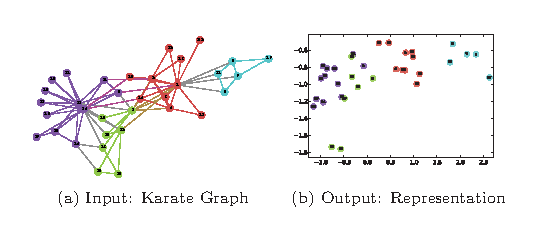
\includegraphics[height=3.8cm]{DeepWalk_1.eps}
    \begin{definition}{Problem Definition}
        Let $G = \left( V ,E \right)$, where $V$ are the members of the network, and $E$ be its edgs.
        Our goal is to learn $X_E\in \mathcal{R} ^{|V|\times d}$, where $d$ is number of 
        latent dimensions.
    \end{definition}
\end{frame}
% 为什么可以套用Word2Vec的思想
\begin{frame}{DeepWalk}
    \centering\includegraphics[height=4cm]{DeepWalk_2.pdf}
    \begin{alertblock}{Connection}
        The power-law distribution of vertices appearing in the short random walks follows 
        a power-law, much like the distribution of words in natural language.
    \end{alertblock}
\end{frame}
% 公式推导
\begin{frame}{DeepWalk}
    \begin{enumerate}
        \item give a sequence of random walk from vertice $i$
            \begin{equation}
                \mathcal{W}_{i}^{n}  = \{v_1, v_2, v_3, \cdots , v_n\}
            \end{equation}
        \item maximize the likehood
            \begin{equation}
                \operatorname{Pr}\left(v_i \mid \left(\Phi(v_1), \Phi(v_2), \cdots, \Phi(v_{i-1}))\right)\right)
            \end{equation}
            \begin{block}{Mapping Function $\Phi$}
                $\Phi: v \in V \longmapsto \mathcal{R}^{|V|\times d}$
                where $d$ is the number of dimensions                
            \end{block}
    \end{enumerate}
\end{frame}
% 为什么使用Skip-Gram
\begin{frame}{DeepWalk}
    \framesubtitle{Disadvantages and Optimizations}
    \begin{itemize}
        \item As the walk length grows, computing this objective function becomes unfeasible.
        \item Restricts the order in which vertices appear
    \end{itemize}
    \centering\includegraphics[height=3.1cm]{DeepWalk_3.pdf}
\end{frame}
% 优化目标与算法
\begin{frame}{DeepWalk}
    \framesubtitle{Algorithm}
    \centering\includegraphics[height=5cm, width=7cm]{DeepWalk_4.pdf}
    \begin{corollary}
        $\underset{\Phi}{\operatorname{minimize}}-\log \operatorname{Pr}\left(\left\{v_{i-w}, \cdots, v_{i-1}, v_{i+1}, \cdots, v_{i+w}\right\} \mid \Phi\left(v_{i}\right)\right)$
    \end{corollary}
\end{frame}
% 结果
\begin{frame}{DeepWalk}
    \framesubtitle{复现结果}
    \begin{table}[]
        \resizebox{\textwidth}{!}
        {
            \begin{tabular}{lllllllllll}
                        & Label Node\% & 10    & 20    & 30    & 40    & 50    & 60    & 70    & 80    & 90    \\
            micro-F1 & 原文结果         & 36.00 & 38.20 & 39.60 & 40.30 & 41.00 & 41.30 & 41.50 & 41.50 & 42.00 \\
                        & 复现结果         & 36.00 & 38.73 & 39.75 & 40.70 & 41.27 & 41.98 & 42.18 & 41.99 & 42.65 \\
            macro-F1 & 原文结果         & 21.30 & 23.80 & 25.30 & 26.30 & 27.30 & 27.60 & 27.90 & 28.20 & 28.90 \\
                        & 复现结果         & 20.90 & 23.78 & 25.33 & 26.31 & 27.09 & 27.84 & 28.16 & 28.25 & 28.78
            \end{tabular}
        }
    \end{table}
\end{frame}
% ---------------------------------------Node2Vec---------------------------------------
\section{Node2Vec}
% 为什么使用BFS与DFS
\begin{frame}{Node2Vec}
    \framesubtitle{Classic Search Strategies}
    \centering\includegraphics[height=3.8cm]{node2vec_1.pdf}
    1. The neighborhoods sampled by BFS lead to embeddings that correspond closely to structural equivalence.\\
    2. DFS can freely explore network neighborhoods which is important in discovering homophilous communities.
\end{frame}
% 如何控制BFS与DFS
\begin{frame}{Node2Vec}
    \framesubtitle{Search Bias $\alpha$ }
    \begin{columns}
        \begin{column}{0.5\textwidth}
            \centering\includegraphics[height=3.6cm]{node2vec_2.pdf}
        \end{column}
        \begin{column}{0.5\textwidth}
            $$
            \alpha_{p q}(t, x)= \begin{cases}\frac{1}{p} & \text { if } d_{t x}=0 \\ 1 & \text { if } d_{t x}=1 \\ \frac{1}{q} & \text { if } d_{t x}=2\end{cases}
            $$
        \end{column}
    \end{columns}
\end{frame}
% 优化目标与算法
\begin{frame}{Node2Vec}
    \framesubtitle{Algorithm}
    \centering\includegraphics[height=5cm]{node2vec_3.pdf}
    \begin{corollary}
        $\max _{f} \sum_{u \in V}\left[\sum_{n_{i} \in N_{S}(u)} f\left(n_{i}\right) \cdot f(u)-\log Z_{u}\right]$
    \end{corollary}
\end{frame}
% ---------------------------------------Stuc2Vec---------------------------------------
\section{Struc2Vec}
% Overview
\begin{frame}{Struc2Vec}
    \centering\includegraphics[height=5cm]{struc2vec.pdf}
    \begin{block}{Limitation}
        Structurally similar nodes will never share the same context if their distance (hop count) is larger than the Skip-Gram window.
    \end{block}
\end{frame}
% 符号解释
\begin{frame}{Struc2Vec}
    \framesubtitle{Structural Similarity}
    \begin{equation}
        \begin{gathered}
        f_{k}(u, v)=f_{k-1}(u, v)+g\left(s\left(R_{k}(u)\right), s\left(R_{k}(v)\right)\right) \\
        k \geq 0 \text { and }\left|R_{k}(u)\right|,\left|R_{k}(v)\right|>0
        \end{gathered}
    \end{equation}
    \begin{alertblock}{符号解释}
        \begin{description}
            \item [$f_k(u, v)$] structural distance when consider k-hop neighborhoods
            \item[$R_{k}(u)$] the ring of nodes at distance k
            \item[$s(S)$] the ordered degree sequence
            \item[$g(a, b)$] DTW Function  
        \end{description}
    \end{alertblock}
\end{frame}
% R, S
\begin{frame}{Struc2Vec}
    \framesubtitle{Example}
    \begin{columns}
        \begin{column}{0.5\textwidth}
            \centering\includegraphics[height=4.6cm]{struc2vec_example.pdf}
        \end{column}
        \begin{column}{0.5\textwidth}
            \begin{example}
                \begin{align*}
                    & R_1(1)=\{2,3,4,6,7\} \\
                    & R_2(1)=\{5,8,9\}\\
                    & s(R_1(1))=\{1,1,1,2,3\}\\
                    & s(R_2(1))=\{1,1,1\} \\
                \end{align*}
            \end{example}
        \end{column}
    \end{columns}
\end{frame}
% DTW
\begin{frame}{Struc2Vec}
    \framesubtitle{DTW}
    \begin{block}{Dynamic Time Warping}
        利用动态规划的思想来计算两条不等长序列的相似度
    \end{block}
    动态转移方程如下:
    $$
    g(i, j) = min\{g(i-1, j),g(i, j-1),g(i-1, j-1)\} + d(i, j)
    $$
    $$d(a, b) = \frac{max(a, b)}{min(a, b)} - 1$$
\end{frame}
% ---------------------------------------LINE--------------------------------------------
\section{LINE}
% 一阶相似度与二阶相似度
\begin{frame}{LINE}
    \framesubtitle{Overview}
    \centering\includegraphics[height=6cm]{line.pdf}
\end{frame}
% 一阶
\begin{frame}{LINE}
    \framesubtitle{First-Order Proximity}
    The Joint Probability between $v_i$ and $v_j$:
    $$p_{1}\left(v_{i}, v_{j}\right)=\frac{1}{1+\exp \left(-\vec{u}_{i}^{T} \cdot \vec{u}_{j}\right)}$$ 
    Empirical Probability $\hat{p}_1(i, j)=\frac{w_{ij}}{W}$
    $$O_{1}=d\left(\hat{p}_{1}(\cdot, \cdot), p_{1}(\cdot, \cdot)\right)$$ 
    where $d(·, ·)$ is the distance between two distributions.
    \begin{block}{Objective Function}
        min $O_{1}=-\sum_{(i, j) \in E} w_{i j} \log p_{1}\left(v_{i}, v_{j}\right)$
    \end{block}
\end{frame}
% 二阶
\begin{frame}{LINE}
    \framesubtitle{Second-Order Proximity}
    The Probability of Context $v_j$ generated by vertex $v_i$ as:
    $$
    p_{2}\left(v_{j} \mid v_{i}\right)=\frac{\exp \left(\vec{u}_{j}^{T} \cdot \vec{u}_{i}\right)}{\sum_{k=1}^{|V|} \exp \left(\vec{u}_{k}^{\prime T} \cdot \vec{u}_{i}\right)}
    $$
    Empirical Probability $\hat{p}_1(v_j \mid v_i)=\frac{w_{ij}}{d_i}$
    \begin{block}{Objective Function}
        $O_{2}=-\sum_{(i, j) \in E} w_{i j} \log p_{2}\left(v_{j} \mid v_{i}\right)$
    \end{block}
\end{frame}
% 优化
\begin{frame}{LINE}
    \framesubtitle{Optimization}
    1. Negative Sample
    $$
    \log \sigma\left(\vec{u}_{j}^{\prime T} \cdot \vec{u}_{i}\right)+\sum_{i=1}^{K} E_{v_{n} \sim P_{n}(v)}\left[\log \sigma\left(-\vec{u}_{n}^{T} \cdot \vec{u}_{i}\right)\right]
    $$
    where $\sigma (x) = \frac{1}{1 + exp(−x)}$ is the sigmoid function.\\
    \hspace*{\fill}\\ 
    \hspace*{\fill}\\ 
    \hspace*{\fill}\\
    2. Edge Sample - Alias Sample
\end{frame}
% -----------------------------------------SDNE-----------------------------------------
\section{SDNE}
\begin{frame}{SDNE}
    \framesubtitle{Overview}
    \centering\includegraphics[height=6cm]{SDNE.pdf}
\end{frame}
% 一阶
\begin{frame}{SDNE}
    \framesubtitle{First-Order Proximity}
    Encoder and Decoder
    $$
    \begin{aligned}
    &\mathbf{y}_{i}^{(1)}=\sigma\left(W^{(1)} \mathbf{x}_{i}+\mathbf{b}^{(1)}\right) \\
    &\mathbf{y}_{i}^{(k)}=\sigma\left(W^{(k)} \mathbf{y}_{i}^{(k-1)}+\mathbf{b}^{(k)}\right), k=2, \ldots, K
    \end{aligned}
    $$
    First-Order Proximity Loss Function
    $$
    \begin{aligned}
    \mathcal{L}_{1 s t} &=\sum_{i, j=1}^{n} s_{i, j}\left\|\mathbf{y}_{i}^{(K)}-\mathbf{y}_{j}^{(K)}\right\|_{2}^{2} \\
    &=\sum_{i, j=1}^{n} s_{i, j}\left\|\mathbf{y}_{i}-\mathbf{y}_{j}\right\|_{2}^{2}
    \end{aligned}
    $$
\end{frame}
% 二阶
\begin{frame}{SDNE}
    \framesubtitle{Second-Order Proximity}
    The autoencoder goal is to minimize:
    $$
    \mathcal{L}=\sum_{i=1}^{n}\left\|\hat{\mathbf{x}}_{i}-\mathbf{x}_{i}\right\|_{2}^{2}
    $$
    {Structural Similarity $x_i=s_i$} 
    $$
    \begin{aligned}
    \mathcal{L}_{2 n d} &=\sum_{i=1}^{n}\left\|\left(\hat{\mathbf{x}}_{i}-\mathbf{x}_{i}\right) \odot \mathbf{b}_{\mathbf{i}}\right\|_{2}^{2} \\
    &=\|(\hat{X}-X) \odot B\|_{F}^{2}
    \end{aligned}
    $$
\end{frame}
% 损失函数
\begin{frame}{SDNE}
    \framesubtitle{Objective Function}
    正则化部分
    $$
    \mathcal{L}_{r e g}=\frac{1}{2} \sum_{k=1}^{K}\left(\left\|W^{(k)}\right\|_{F}^{2}+\left\|\hat{W}^{(k)}\right\|_{F}^{2}\right)
    $$
    损失函数
    $$
    \begin{aligned}
    \mathcal{L}_{m i x} &=\mathcal{L}_{2 n d}+\alpha \mathcal{L}_{1 s t}+\nu \mathcal{L}_{r e g} \\
    &=\|(\hat{X}-X) \odot B\|_{F}^{2}+\alpha \sum_{i, j=1}^{n} s_{i, j}\left\|\mathbf{y}_{i}-\mathbf{y}_{j}\right\|_{2}^{2}+\nu \mathcal{L}_{r e g}
    \end{aligned}
    $$
\end{frame}
% -----------------------------------------END------------------------------------------
\end{document}